\section{Multimedia Representation and Perception}




\begin{questionbox}{Domanda 1}
Explain the \textbf{Contrast Sensitivity Function} (\textbf{CSF}): what it is, in which units \textbf{spatial frequency} is measured, where it peaks, and the direct implication for \textbf{quantization} in compression.
\end{questionbox}


\begin{itemize}
  \item \textbf{\textbf{CSF}}: HVS sensitivity to luminance contrast as \textbf{spatial frequency} changes.
  \item Unit: \textbf{cycles per degree} of visual angle.
  \item Shape: band-pass → low sensitivity at very low and very high frequencies; peak at intermediate frequencies.
  \item Compression consequence → frequency-dependent \textbf{quantization}:
  \item visually important frequencies → smaller steps;
  \item less visible frequencies → coarser steps.
\end{itemize}



\begin{questionbox}{Domanda 2}
Compare \textbf{cones} and \textbf{rods} (number, function, lighting conditions) and explain why the RGB-to-Y conversion weights the green component the most.
\end{questionbox}


\begin{itemize}
  \item \textbf{\textbf{rods}}: high light sensitivity, low-light vision, no color.
  \item \textbf{\textbf{cones}}: color vision, brighter conditions, short/medium/long wavelength classes.
  \item Luminance example:
\end{itemize}


$$
Y \approx 0.299R + 0.587G + 0.114B
$$


\begin{itemize}
  \item Green coefficient largest → HVS most sensitive to green/yellow luminance detail.
\end{itemize}



\begin{questionbox}{Domanda 3}
Explain the J:a:b \textbf{\textbf{chroma} subsampling} notation. Compute the data-reduction factor of 4:2:0 vs full RGB and justify why it is perceptually acceptable.
\end{questionbox}


\begin{itemize}
  \item $J:a:b$ → \textbf{chroma} samples kept relative to $J$ \textbf{luma} samples over two rows.
  \item 4:2:0 → full-resolution $Y$, half horizontal and half vertical $Cb,Cr$.
  \item Over $2\times2$ pixels:
  \item RGB: $4\times3=12$ component samples;
  \item YCbCr 4:2:0: $4Y+1Cb+1Cr=6$ component samples.
  \item Reduction → about $1/2$ of full RGB component samples.
  \item Perceptual reason → eye is more sensitive to luminance detail than chrominance detail.
\end{itemize}



\begin{questionbox}{Domanda 4}
Draw the Basic Tools for Compression scheme (Transform -> Prediction -> \textbf{quantization} -> \textbf{entropy} Coding) and indicate which stage is the only \textbf{lossy} one and why.
\end{questionbox}


\begin{figure}[H]
\centering
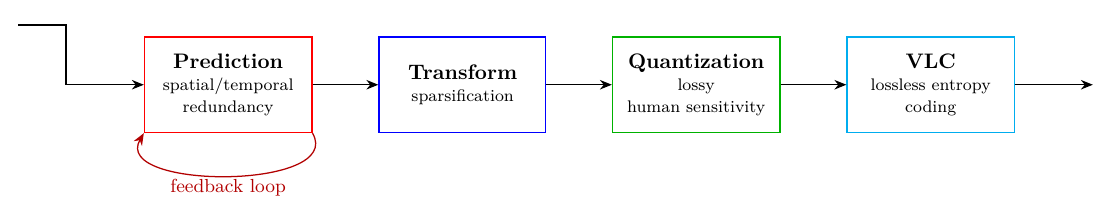
\includegraphics[width=0.75\textwidth]{images/Pasted_image_20260624205523.png}
\caption{Pasted image 20260624205523}
\end{figure}\begin{tcolorbox}[colback=white, colframe=gray!50, height=4.5cm, sharp corners]
\end{tcolorbox}

\begin{itemize}
  \item Prediction / transform → decorrelate signal or compact energy.
  \item \textbf{entropy} coding → \textbf{lossless}; shorter codes for more probable symbols.
  \item \textbf{\textbf{quantization}} → only \textbf{lossy} stage: many input values map to same reconstruction value → exact original cannot be recovered.
\end{itemize}

---


